\documentclass[12pt,A4,A4pt]{article}

\usepackage{amsmath}
\renewcommand*\familydefault{\sfdefault} 
\usepackage[scaled]{helvet}
\renewcommand\familydefault{\sfdefault} 
\usepackage[T1]{fontenc}
%\usepackage[T1]{fontenc}
%\usepackage{arial} 
%\pagestyle{myheadings}{}
 %\markboth{left head}{right head}
\usepackage{amssymb}
%\usepackage{epsfig}
\usepackage{fancyhdr}
\usepackage{float}
%\usepackage[authoryear,round]{natbib}
%\usepackage{apacite}
\usepackage{natbib}
%\usepackage[sort&compress]{natbib}
\usepackage[pdftex]{graphicx}
\usepackage{color}
\usepackage[brazil]{babel}
\usepackage[utf8]{inputenc}
\usepackage{amsfonts}
\usepackage{textcomp}
\usepackage{tabularx}
\usepackage{multirow}
\usepackage{times}
\usepackage{multicol}
\usepackage{lscape}
\usepackage{subfig}
\usepackage{epstopdf}
\usepackage{setspace}
\usepackage{fancyhdr}
\usepackage{epigraph}
\usepackage{scrextend}
\usepackage[shortlabels]{enumitem}
\usepackage{ragged2e}

%\let\OLDthebibliography\thebibliography
%\renewcommand\thebibliography[1]{\OLDthebibliography{#1} \setlength{\parskip}{0pt}\setlength{\itemsep}{0pt plus 0.3ex}}

%\renewcommand{\chaptermark}[1]{\markboth{\MakeUppercase{#1}}{}}
%\renewcommand{\sectionmark}[1]{\markright{\MakeUppercase{#1}}{}}
\pagestyle{fancy}
\fancyhf{}
\renewcommand{\headrulewidth}{0cm}
%\renewcommand{\footrulewidth}{0}
\usepackage{pdfpages}
\usepackage{stackrel}
\usepackage[left=3cm, right=3cm, top=2.5cm, bottom=2.5cm]{geometry}
\newtheorem{exemplo}{Exemplo}
\newtheorem{definicao}{Definição}
\newtheorem{teorema}{Teorema}
\cfoot{{\fontsize{10pt}{\baselineskip}\selectfont \textbf{8\textsuperscript{o} MCSul / VIII SEMENGO - Universidade Federal do Rio Grande}}}

%%%%%
%tira os numeros da frente do autor
\makeatletter 
\renewcommand\@biblabel[1]{}
\makeatother
%%

\begin{document}
\pretolerance10000

\begin{figure}
\centering
\vspace{-1cm}
\begin{minipage}[c]{\textwidth}
\centering
    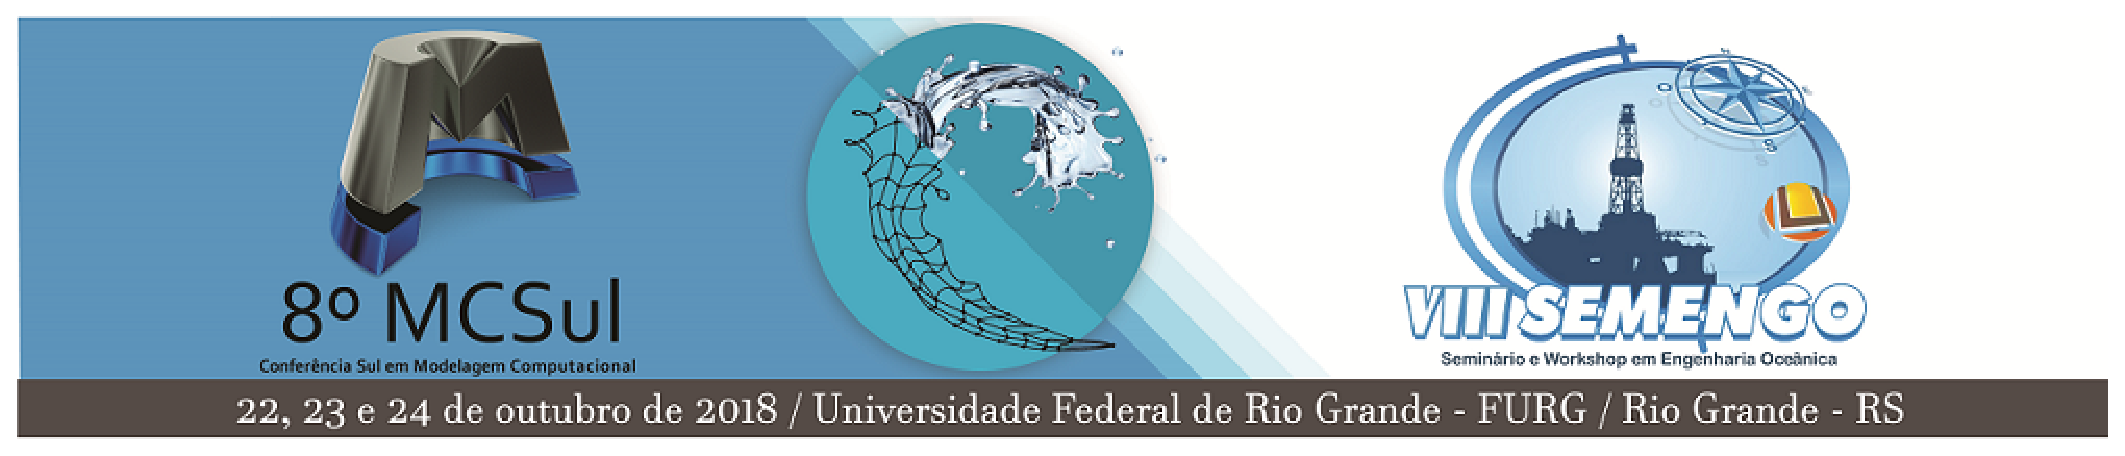
\includegraphics[width=6.2in]{cabecalho.eps}
\end{minipage}
\end{figure}

\begin{center}
\fontsize{16pt}{\baselineskip}\selectfont 
\textbf{{AVALIAÇÃO DE DESEMPENHO DO ALGORITMO DE EVOLUÇÃO DIFERENCIAL ASSOCIADO AO DESIGN CONSTRUTAL PARA A OTIMIZAÇÃO DE UMA CAVIDADE EM FORMA DE DUPLO-T}}
\end{center}
\vspace{-0.9cm}
% \begin{center}
% \vspace{0.5cm}
% \textbf{\large{\textit{TÍTULO DO TRABALHO EM INGLÊS}}}
% \end{center}

\begin{flushright}
Gill V. Gonzales\footnote{Mestre, Instituto Federal Sul-Rio-Grandense - Campus Santana do Livramento, RS, Brazil, gillgonzales@ifsul.edu.br.}$^{,2}$

Liércio A. Isoldi\footnote{Doutor, Universidade Federal do Rio Grande - PPG em Modelagem Computacional, Rio Grande, RS, Brazil, liercioisoldi@furg.br.}

Luiz A. Oliveira Rocha\footnote{Doutor, Universidade do Vale do Rio dos Sinos - PPG em Engenharia Mecânica – São Leopoldo, RS, Brasil luizor@unisinos.br.}

Elizaldo D. dos Santos\footnote{Doutor, Universidade Federal do Rio Grande - PPG em Modelagem Computacional, Rio Grande, RS, Brazil, elizaldosantos@furg.br.}

Antônio J. Silva Neto\footnote{Doutor, Universidade do Estado do Rio de Janeiro, Instituto Politécnico, Nova Friburgo, RJ, Brazil, ajsneto@iprj.uerj.br.}

\end{flushright}

\begin{flushleft}
{\small \setstretch{0.5} \justify
\textbf{Resumo:} Neste trabalho é investigado o desempenho do algoritmo de Evolução Diferencial  associado ao método Design Construtal para a otimização geométrica de um problema de transferência de calor. O problema consiste em uma cavidade em forma de Duplo-T inserida em um sólido com geração de calor constante e uniforme. Portanto, a geometria da cavidade afeta diretamente a performance térmica do problema, definida através do valor da temperatura máxima em excesso, o qual se pretende minimizar. A definição dos graus de liberdade e restrições do problema de otimização é realizada através do método de Design Construtal. O algoritmo de Evolução Diferencial é empregado no processo de otimização. Neste estudo, são avaliados os parâmetros do algoritmo, tais como o operador de mutação, taxa de cruzamento, fator de amplificação do cálculo diferencial e número de iterações. O número de iteração está relacionado aos parâmetros que configuram o número de gerações e quantidade de indivíduos na população.  O objetivo principal do trabalho é avaliar os parâmetros do algoritmo de Evolução Diferencial e qual a influência na correta reprodução dos efeitos dos graus de liberdade sobre a geometria ótima e performance térmica do problema. A principal contribuição do trabalho é a recomendação de um conjunto de parâmetros adequados que adaptem o algoritmo de Evolução Diferencial ao problema estudado. Os resultados indicam como mais influentes os parâmetros de taxa de cruzamento e fator de amplificação, sendo mais adequados os  respectivos valores de 0.7 e 1.5. Estes parâmetros tornaram os resultados do algoritmo de Evolução Diferencial mais robustos e necessitando de um menor número de avaliações da função objetivo para a obtenção das geometrias ótimas.

\vspace{0.3cm}

\noindent\textbf{Palavras-chave:} Otimização Geométrica. Transferência de Calor. Design Construtal. Evolução Diferencial.}
\end{flushleft}

% \noindent\textbf{Abstract:} O resumo em inglês apresenta-se logo após o resumo em português. Sugere-se encaminhar o texto para ser traduzido por um profissional. Caso o artigo esteja em inglês, deve haver uma versão do título, resumo e palavras-chave em português ou espanhol.
% \vspace{0.3cm}

% \noindent\textbf{Keywords:} Keywords. Keywords. Keywords. Keywords. Keywords.}

\newpage
 \onehalfspacing
\section{Introdução}

 {\fontsize{12pt}{\baselineskip}\selectfont}
 
\hspace{0.5cm}A pesquisa em cavidades resfriadoras têm início no trabalho de \cite{Biserni2004}, onde são propostas as formas elementares C e T. Neste trabalho \citep{Biserni2004}, o método de Design Construtal é aplicado para a definição do problema de otimização, assim como a avaliação da influência da geometria sobre a minimização da resistência térmica entre a cavidade e o sólido. O método Design Construtal é um método de restrições e objetivos utilizado para mostrar que o design em sistemas de fluxo/escoamento de dimensões finitas é obtido a partir de um princípio físico de maximização do acesso das correntes internas ao longo do domínio do sistema denominado de Lei Construtal. A Lei Construtal afirma que "Para um sistema de escoamento, animado ou inanimado, evoluir no tempo (sobreviver) é preciso que sua forma e estrutura também evoluam de forma a facilitar a passagem do fluxo" \citep{Bejan}. Portanto, a geometria é o resultado de um processo de otimização da passagem do escoamento. É importante salientar que o método de Design Construtal (DC) não é o método de otimização. O DC determina os graus de liberdade, restrições e espaço de busca do problema para a avaliação da geometria. Para a otimização geométrica são aplicados métodos de otimização como a Busca Exaustiva, onde são avaliadas todas as soluções factíveis, ou métodos heurísticos baseados em processos estocásticos, como o Algoritmo Genético (AG) ou o método de Recozimento Simulado (RS) \citep{Lorenzini2014,Gonzales2015energy}.

\cite{Biserni2004} concluiu que a cavidade em forma de T é mais eficiente que a primeira forma elementar em C, pois consegue adentrar melhor no domínio computacional investigado distribuíndo de forma mais homogênea o campo de temperaturas dentro do domínio sólido. A partir desta observação, formas mais complexas são investigadas na literatura recente \citep{Biserni2007,Lorenzini2011,Lorenzini2014,Biserni2017,Xie2010}. Por exemplo, no trabalho de \cite{Lorenzini2011} a cavidade proposta em forma de Y, foi até 66\% mais eficiente que a forma elementar C. Portanto, na literatura recente, é possível constatar que formas mais complexas possuem um maior desempenho na minimização da resistência térmica entre o sólido e a cavidade, para as mesmas condições térmicas e restrições. Este comportamento só é observado em problemas com elevada intensidade de fluxo/escoamento na cavidade. Entretanto, quanto maior a complexidade da cavidade maior é o esforço computacional necessário no processo de otimização geométrica, principalmente quando o método de otimização empregado é o método de Busca Exaustiva (BE), quando todas as possibilidades geométricas são simuladas. Neste sentido, com a proposta de minimização do esforço computacional e possibilidade de investigar outras características do problema, métodos heurísticos são utilizados no processo de otimização \citep{Lorenzini2014, Gonzales2015energy, Gonzales2017, Biserni2017}.

O uso de métodos heurísticos requer a configuração de parâmetros que controlam o comportamento destes métodos durante o processo de busca pela solução ótima. No trabalho de \cite{Gonzales2015energy} foi empregado o algoritmo de Recozimento Simulado (RS) para a otimização geométrica da cavidade em forma de Y. Este estudo mostrou como um parâmetro de configuração do método pode influenciar os resultados, como por exemplo, o efeito dos graus de liberdade sobre a minimização da temperatura máxima em excesso. O parâmetro analisado foi a função que controla o decaimento da temperatura do RS durante as iterações do algoritmo. Diferentes parâmetros foram investigados e identificados aqueles que levaram ao melhor ou pior desempenho. O parâmetro identificado como $Fast$, por exemplo, apresentou os piores resultados e influenciaria negativamente a avaliação geométrica caso seus resultados fossem utilizados. 

No trabalho de \cite{Gonzales2017} foram comparadas duas diferentes meta-heurísticas, RS e Luus-Jaakola (LJ), e também diferentes versões destes métodos, variando seus parâmetros. Este estudo compara estatisticamente o desempenho dos algorítimos em encontrar a geometria ótima na otimização da cavidade em forma de Duplo-T. Neste estudo, o algoritmo RS, com a função híbrida de decaimento de temperatura, identificada como $BoltzExp$, apresentou os melhores resultados entre os métodos investigados. No trabalho de \cite{Gonzales2018}, foi realizada uma comparação entre os algortimos de Evolução Diferencial (ED) e RS, baseada na análise estatística em encontrar a geometria ótima para o problema investigado em \cite{Gonzales2017}. Neste estudo, os resultados do algoritmo ED foram superiores aos resultados do algoritmo RS.

Neste artigo, será investigada a aplicação do algoritmo de ED na otimização geométrica da cavidade em forma de Duplo-T. Serão comparados os resultados de diferentes versões do algoritmo ED, configurados com diferentes parâmetros, assim como, com diferentes iterações. Portanto, diferente dos estudos da literatura recente relatados \citep{Gonzales2017, Gonzales2018}, este trabalho propõe uma análise estatística focada na reprodução dos efeitos da geometria ótima sobre a temperatura máxima em excesso adimensional do domínio computacional, e não apenas na obtenção da configuração geométrica ótima ou minimização da resisência térmica.

\section{Modelagem Matemática e Numérica}
\label{modelo}
\hspace{0.5cm}A Figura \ref{figure01} apresenta o sólido em um domínio bidimensional, com a terceira dimensão $W$, perpendicular ao plano da figura. O domínio sólido é representado pela região cinza na Fig. \ref{figure01}, a qual possui uma geração de calor interna constante e uniforme a uma taxa volumétrica dada por $q^{'''}(Wm^{\tiny -3})$. O sólido possui uma condutividade térmica constante $k$. As superfícies externas do sólido estão perfeitamente isoladas (adiabática). Neste caso, o calor só pode ser removido através da cavidade em forma de Duplo-T, que está mantida a uma temperatura mínima $(\theta_{min})$. A temperatura mínima da cavidade representa idealmente o escoamento de um fluido refrigerante em mudança de fase a baixa temperatura escoando pela região da cavidade. Nestes casos, o coeficiente de transferência de calor na parede da cavidade é assumido tão grande que a resistência convectiva pode ser negligenciada em comparação com a resistência condutiva do sólido. 

\begin{figure}[h!]
\centering
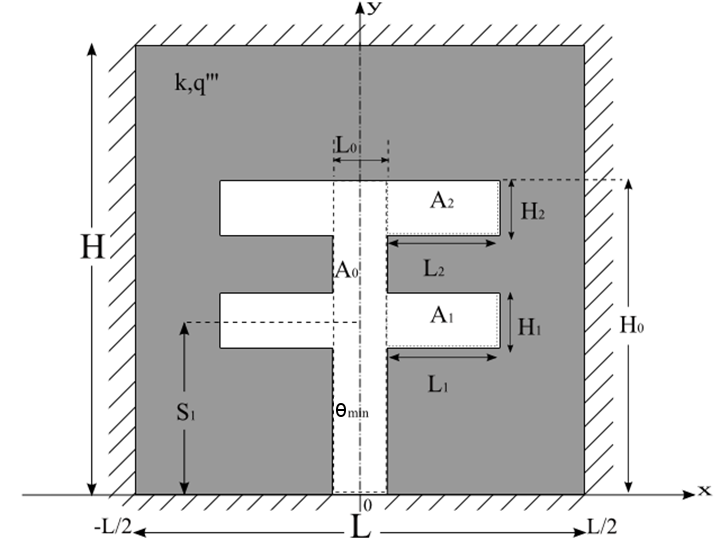
\includegraphics[width=0.6\linewidth]{imgs/duplo_t.png}
\caption{ {\small Domínio Computacional da Cavidade em Forma de Duplo-T.}}
\label{figure01}
\end{figure}

O objetivo da análise é determinar a geometria ótima ($H/L$, $H_{0}/L_{0}$, $H_{1}/L_{1}$, $H_{2}/L_{2}$ e $S_{1}/H_{0}$) que minimiza a máxima temperatura em excesso adimensional $(\theta_{max} - \theta_{min})/(q^{'''}A)$. De acordo com o DC esta otimização deve ser submetida as restrições de área total e cavidade, representadas, respectivamente, pelas seguintes equações:

\begin{equation}
A = HL \label{area_total}
\end{equation}
\begin{equation}
A_{c} = A_{0} + 2A_{1} + 2A_{2} \label{area_cavidade}
\end{equation}
A fração da área da cavidade em relação a área total é dada por:
\begin{equation}
\phi_{c} = A_{c}/A \label{fi}
\end{equation}
Para a determinação do campo de temperaturas no domínio sólido, é necessário resolver a equação da condução do calor, dada  na sua forma adimensional por:
\begin{equation}
\frac{\partial^{2} \theta}{\partial \tilde{x}^{2}}+\frac{\partial^{2} \theta}{\partial \tilde{y}^{2}}+1=0 \label{calor}
\end{equation}

onde as variáveis adimensionais são dadas por:

\begin{equation}
\tilde{\theta} = \frac{\theta - \theta_{min}}{q^{'''}\cdot\frac{A}{k}}\label{tadim}
\end{equation}

\begin{equation}
\tilde{x},\tilde{y},\tilde{H}_{0},\tilde{H}_{1},\tilde{H}_{2},\tilde{L}_{0},\tilde{L}_{1},\tilde{L}_{2},\tilde{H},\tilde{L},\tilde{S}_{1} = \frac{x,y,H_{0},H_{1},H_{2},L_{0},L_{1},L_{2},H,L,S_{1}}{A^{1/2}}\label{vadim}
\end{equation}

Por razões de brevidade, as equações das condições de contorno de fluxo nulo nas superfícies externas ao sólido, bem como, as equações de condições de contorno de temperatura mínima nas paredes da cavidade não são apresentadas, podendo ser vistas no trabalho de  \cite{Gonzales2015cilamce}. Será usada a notação $Nm$ para a temperatura máxima em excesso adimensional $N$ vezes minimizada, por exemplo $(\tilde{\theta} _{max})_{4m}$ para quatro vezes. Da mesma forma, será usado um numerador seguido da letra $o$ para o grau de liberdade otimizado, por exemplo, para $H_{1}/L_{1}$ duas vezes otimizado $(H_{1}/L_{1})_{2o}$.

A forma adimensional das Eqs. \ref{area_total}-\ref{area_cavidade} são representadas pelas seguintes equações:

\begin{equation}
1  = \tilde{H}\tilde{L}\label{total_area_adim}
\end{equation}
\begin{equation}
\phi_{c}=\tilde{H}_{0}\tilde{L}_{0}+2\phi_{1}+2\phi_{2}\label{fi_c}
\end{equation}
\begin{equation}
\phi_{1}=\tilde{H}_{1}\tilde{L}_{1}\label{fi_1}
\end{equation}
\begin{equation}
\phi_{2}=\tilde{H}_{2}\tilde{L}_{2}\label{fi_2}
\end{equation}

O objetivo é minimizar o máximo excesso de temperatura adimensional representado pela seguinte equação:

\begin{equation}
\tilde{\theta}_{max}=\frac{\theta_{max}-\theta_{min}}{q^{'''}\cdot\frac{A}{k}}\label{fo}
\end{equation}

Para a determinação da $(\tilde{\theta}_{max})_{5m}$ é necessário a otimização de cinco graus de liberdade ($H/L$, $H_{0}/L_{0}$, $H_{1}/L_{1}$, $H_{2}/L_{2}$ e $S_{1}/H_{0}$) submetidos as restrições de área da cavidade ($\phi_{c}$, $\phi_{1}$ and $\phi_{2}$) e de área total do sólido.

A função representada pela Eq. \ref{fo} é resolvida numericamente através da  solução da equação da difusão do calor, Eq. \ref{calor}, para determinar os campos de temperatura em todo o domínio computacional para diferentes configurações de ($H/L$, $H_{0}/L_{0}$, $H_{1}/L_{1}$, $H_{2}/L_{2}$ e $S_{1}/H_{0}$) e calculando o $\tilde{\theta}_{max}$ para minimizar o seu valor através da variação da configuração geométrica. A solução numérica é dada pela aplicação do Método de Elementos Finitos (FEM), baseado em elementos finitos triangulares, desenvolvido no ambiente MATLAB, com o pacote PDE (partial-differential-equations) toolbox \citep{Reddy1994}. A malha é não-uniforme em ambos eixos $x$ e $y$, e varia de uma geometria para outra. O tamanho apropriado da malha é determinado por sucessivos refinamentos de malha (h-adaptativo), aumentando o número de elementos quatro vezes a cada refinamento. Por questões de simplicidade, o teste de malha independente pode ser verificado no trabalho de \cite{Gonzales2015cilamce}.

\section{Otimização Geométrica}
\label{opt}
\hspace{0.5cm}A otimização geométrica da cavidade em forma de Duplo-T é realizada através da variação das variáveis que definem a geometria da cavidade e, de acordo com o método DC, este processo é sujeito a restrições. Entretanto, a cavidade estudada neste trabalho possui nove variáveis ($H$, $L$, $H_{0}$, $L_{0}$, $H_{1}$, $L_{1}$, $H_{2}$, $L_{2}$ e $S1$) e quatro restrições ($A$, $\phi_{c}$, $\phi_{1}$ e $\phi_{2}$), então são necessários cinco graus de liberdade (GL) para o fechamento das equações e determinar a geometria ($H/L$, $H_{0}/L_{0}$, $H_{1}/L_{1}$, $H_{2}/L_{2}$ e $S_{1}/H_{0}$). O processo de otimização está concentrado em quatro GLs ( $H_{0}/L_{0}$, $H_{1}/L_{1}$, $H_{2}/L_{2}$ e $S_{1}/H_{0}$), sendo $H/L$ variado em diferentes valores entre $0.03< H/L >30$ e as demais restrições mantidas em $A$ = 1, $\phi_{c}=0.1$; $\phi_{1} =0.015$; $\phi_{2}=0.015$. Em razão da brevidade, as equações que demonstram a definição das variáveis em função dos graus de liberdade podem ser verificados no trabalho de \cite{Gonzales2015cilamce}.


%\subsection{Constructal Design}
%\label{ed}
%\hspace{0.5cm}A otimização geométrica...


\subsection{Evolução Diferencial}
\label{ed}
\hspace{0.5cm}O algoritmo de Evolução Diferencial (ED) é uma meta-heurística baseada em populações e computação evolutiva. Foi proposto originalmente no trabalho de \cite{Storn1997}, principalmente para espaços contínuos. O algoritmo ED foi projetado para ter habilidade com funções de custo não lineares, não diferenciáveis e multimodal \citep{Storn1997}. A vantagem deste método está em possuir poucos parâmetros de controle, pode ser adaptado a computação paralela e possui boas propriedades de convergência \citep{Storn1997}. O algorítimo é baseado em dois laços aninhados. O primeiro laço determina as gerações. O segundo laço, interno ao primeiro, é responsável pela aplicação de operadores diferenciais na população de soluções, com o objetivo de gerar uma nova população com indivíduos evoluídos, melhores soluções. Cada membro da população de soluções representa uma solução factível do problema. Esta solução deve ser um vetor com tamanho igual a dimensão do problema. O tamanho da população ($NP$), é definida a priori e não muda durante o processo de otimização, segundo a definição clássica. Para a geração da primeira população é necessária uma distribuição uniforme cobrindo todo o espaço de busca. Logo, em cada geração e para cada vetor solução, um novo vetor é criado através da perturbação de um vetor, escolhido aleatoriamente, com a diferença entre dois outros vetores, também escolhidos de forma aleatória. O novo vetor gerado é chamado de vetor mutante. Este processo representa o operador de mutação do algorítimo ED, o qual é aplicado para todos os indivíduos da população $x_{i,G}$, $i = 1,2,3...NP$. A seguinte equação representa o operador de mutação:

\begin{equation}
v_{i,G+1} = x_{r_{1},G} + F . (x_{r_{2},G} - x_{r_{3},G}) \label{trial}
\end{equation}

onde os índices $r_{1}$, $r_{2}$, $r_{3}$ $\in \{1,2,3 ...NP\}$, são aleatórios, inteiros e mutuamente diferentes. Os valores de $r_{1}$, $r_{2}$ e $r_{3}$ devem ser diferentes do índice do indivíduo da iteração atual. O parâmetro $F$ é um fator constate de valor real $\in [0,2]$ que controla a amplitude da variação diferencial $(x_{r_{2},G} - x_{r_{3},G})$. O operador de mutação apresentado é chamado pelos autores de rand/1/bin. Um segundo tipo de operador de mutação é utilizado e identificado pelos autores como best/2/bin \citep{Storn1997}. Neste operador são usados dois vetores a mais no cálculo diferencial ($x_{r3}$ e $x_{r4}$), bem como, a soma da diferença entre os vetores aleatórios com a melhor solução encontrada até a geração $G$ atual ($x_{{best},G}$). O uso de mais dois vetores no operador diferencial aumenta a diversidade da solução mutada \citep{Storn1997}. A equação abaixo representa o operador de mutação best/2/bin:

\begin{equation}
v_{i,G+1} = x_{{best},G} + F . (x_{r_{1},G} + x_{r_{2},G} - x_{r_{3},G} - x_{r_{4},G}) \label{trial2}
\end{equation}


Além dos operadores apresentados, o algoritmo ED possui o operador de cruzamento. Este operador aumenta a diversidade da solução mutante e cria o vetor candidato a ser integrado na nova população, o vetor $trial$. O vetor $trial$ é aceito como um novo membro da população substituindo o indivíduo atual na iteração $i$, apenas se a solução é melhor. Outros dois parâmetros configuram o comportamento do ED, sendo eles o tamanho da população $NP$ e a quantidade de gerações $G$. O critério de parada do algorítimo é determinado a priori pelo número total de gerações. Por razões de simplificação, maiores detalhes sobre o algorítimo ED podem ser verificados em \cite{Storn1997}.

Neste trabalho, quatro diferentes versões do algorítimo ED foram executadas com diferentes parâmetros de mutação, cruzamento $CR$ e fator de amplificação $F$. Os valores investigados para $CR$ e $F$ estão de acordo com a faixa de  valores recomendada pelos autores do método \citep{Storn1997}. Além destes parâmetros, para cada versão do algoritmo, foram configuradas diferentes combinações de tamanho da população e número de gerações a serem processadas. A versão nomeada como ED1 possui a taxa de cruzamento  configurada igual a $0.7$ e fator $F = 1.5$. A segunda versão, chamada ED2, possui $CR = 0.9$ e $F = 2$. As versões ED3 e
ED4, possuem respectivamente as mesmas configurações das versões ED1 e ED2. Contudo, ED3 e ED4 possuem o operador de mutação best/2/bin. A Tabela \ref{tab:algos} apresenta todas as variações do algoritmo ED estudadas neste trabalho.

\begin{table}[htbp]
\small
\centering
\caption{\small Configurações das Diferentes Versões do Algorimo ED Analisadas}
\begin{tabular}{cccc}
\hline
Algoritmo & Mutação & $CR$ & $F$ \\
\hline
ED1 & $rand/1/bin$ & $0.7$ & $1.5$  \\
ED2 & $rand/1/bin$ & $0.9$ & $2$  \\
ED3 & $best/2/bin$ & $0.9$ & $2$  \\
ED4 & $best/2/bin$ & $0.7$ & $1.5$  \\
\hline
\end{tabular}
  \label{tab:algos}
\end{table}

A Tabela \ref{tab:popgeracao} apresenta as diferentes combinações de tamanho da população e gerações configuradas para cada versão do algoritmo ED.

\begin{table}[htbp]
\small
\centering
\caption{\small Combinações dos Parâmetros de Tamanho da População $(NP)$ e Número de Gerações $(G)$}
\begin{tabular}{ccc}
\hline
$(NP)$ & $(G)$ & Total de Iterações \\
\hline
$5$ & $10$ & $50$	\\
$10$ & $10$ & $100$	\\
$10$ & $15$ & $150$	\\
$15$ & $20$ & $300$	\\
\hline
\end{tabular}
  \label{tab:popgeracao}
\end{table}

\section{Resultados}
\label{opt}
\hspace{0.5cm}Na Figura \ref{destdinner} são apresentados os resultados da otimização geométrica de 4 Graus de Liberdade (GL) ($H_{0}/L_{0}$, $H_{1}/L_{1}$, $H_{2}/L_{2}$ e $S_{1}/H_{0}$) para diferentes valores de $H/L$. Foram executadas 30 rodadas de cada versão do algoritmo de ED para diferentes combinações de $NP$ e $G$, sendo registrados os valores de $({\tilde{\theta}}_{max})_{4m}$ encontrados durante cada processo de otimização. 

\begin{figure}[htbp]
\centering
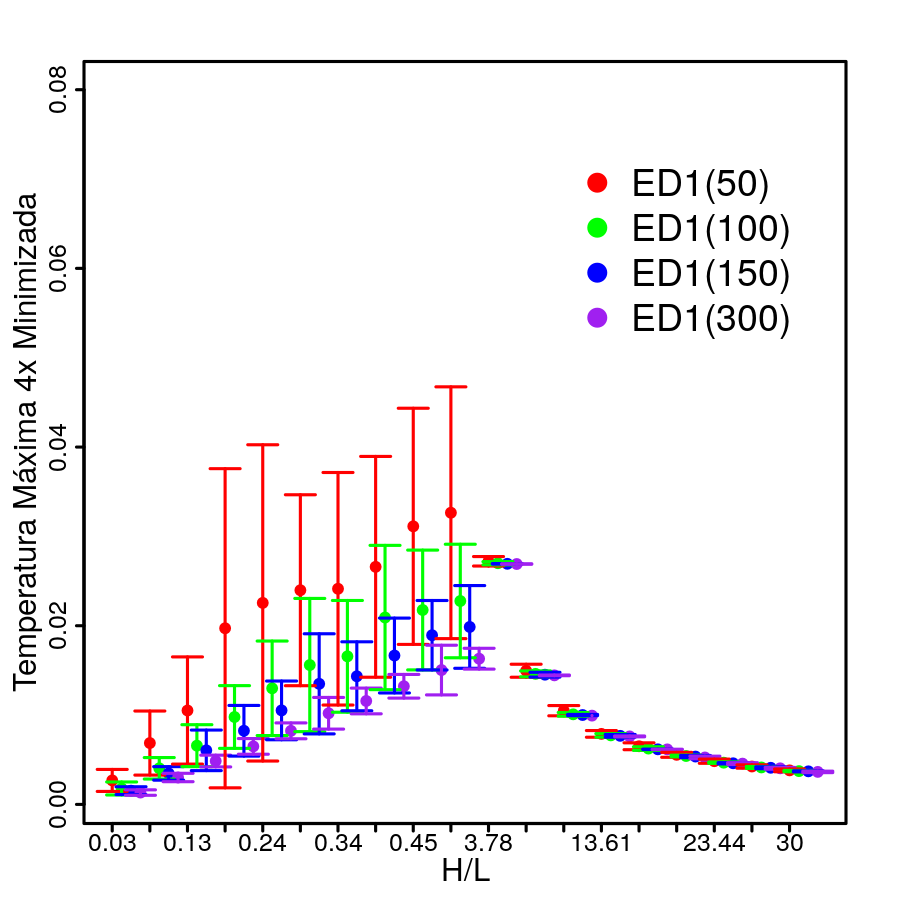
\includegraphics[scale=.98]{imgs/plot_de1_rdata_std.png}
\quad
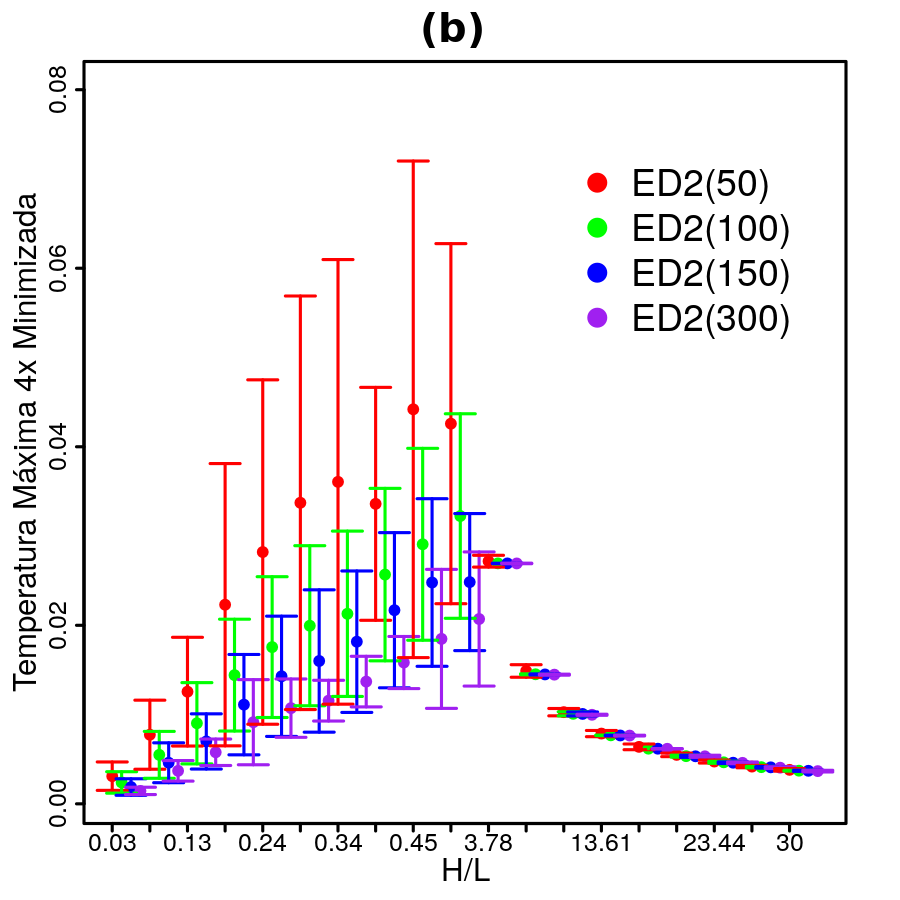
\includegraphics[scale=.98]{imgs/plot_de2_rdata_std.png}
\quad
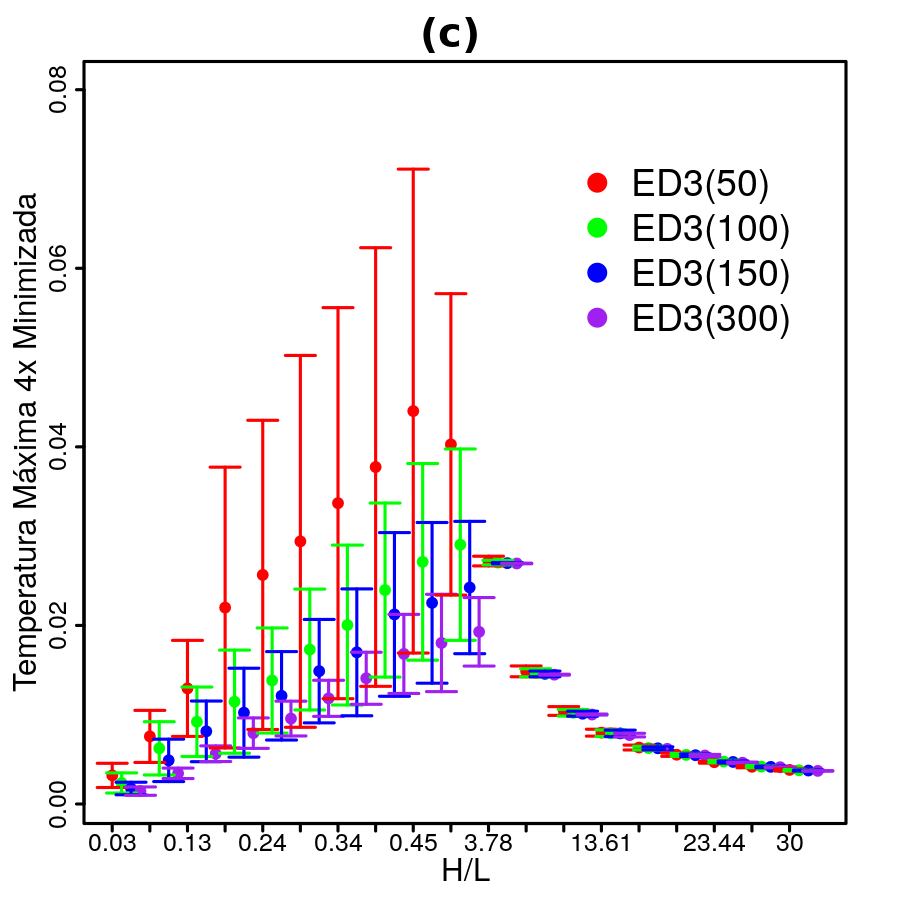
\includegraphics[scale=.98]{imgs/plot_de3_rdata_std.png}
\quad
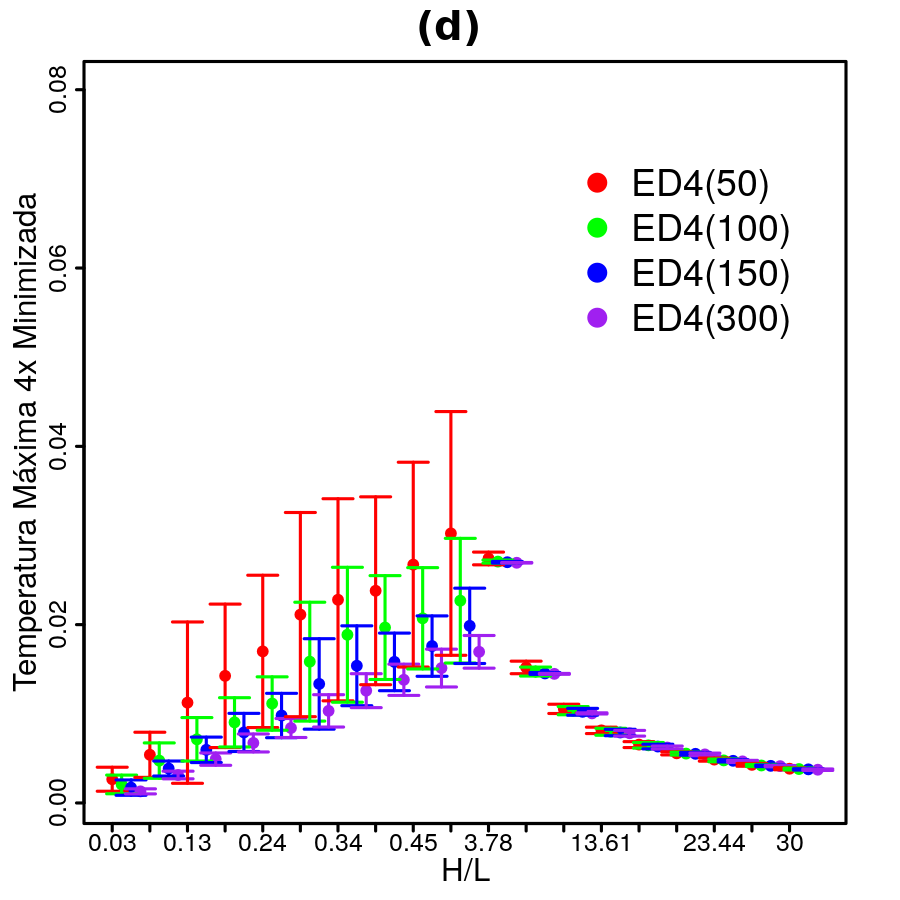
\includegraphics[scale=.98]{imgs/plot_de4_rdata_std.png}

\caption{\fontsize{10pt}{\baselineskip}\selectfont Média e Desvio Padrão do Efeito de $H/L$ sobre $({\tilde{\theta}}_{max})_{4m}$ registrados por diferentes versões do algoritmo ED com diferentes combinações de população e gerações: a)ED1 b)ED2 c)ED3 d)ED4.}
\label{destdinner}
\end{figure}

A Figura \ref{destdinner} apresenta a média e o desvio padrão em relação ao efeito de $H/L$ sobre $({\tilde{\theta}}_{max})_{4m}$. Na Fig. \ref{destdinner}, é possível observar que para as razões de $H/L>0.5$, todos os algoritmos apresentam um desvio padrão muito pequeno, independente inclusive do número de iterações ($NP \times G$). Este comportamento é devido ao espaço de busca do problema, que nesta região ($H/L>0.5$) possui poucos mínimos locais, facilitando a convergência do algoritmo, independente de sua configuração. Este resultado é importante, pois indica que a configuração do algoritmo e o esforço computacional pode ser adaptado de acordo com o espaço de busca. 
Para razões de $H/L\leqslant0.5$, todas as versões do algoritmo ED analisadas neste estudo obtiveram alguma dificuldade em convergir para o ótimo, apresentando erros identificados pelo desvio padrão. Nestes casos, a influência dos parâmetros de configuração do algoritmo ED se torna mais evidente. A Fig. \ref{destdinner} apresenta, em cada gráfico, uma comparação dentro de cada versão do algoritmo ED, variando apenas o número de iterações ($NP \times G$). Portanto, é possível notar a influência dos parâmetros de $NP$ e $G$ na redução do desvio padrão. Porém, obviamente, as melhores configurações destes dois parâmetros são aquelas que demandam um maior custo computacional. Entretanto, é preciso destacar que as versões ED1 e ED4 possuem menor desvio padrão para o algoritmo com 50 iterações em comparação com os demais algoritmos. O aumento no tamanho da população e número de gerações para 300 iterações, reduz significativamente o desvio padrão nestas versões do algorimo ED, como pode ser observado nas Figs. \ref{destdinner}(a) e \ref{destdinner}(d). Por outro lado, nas Figs. \ref{destdinner}(b) e \ref{destdinner}(c) a diferença no desvio padrão é maior e o aumento do número de iterações também não representa diminuição significativa do desvio padrão.

\begin{figure}[!htbp]
\centering
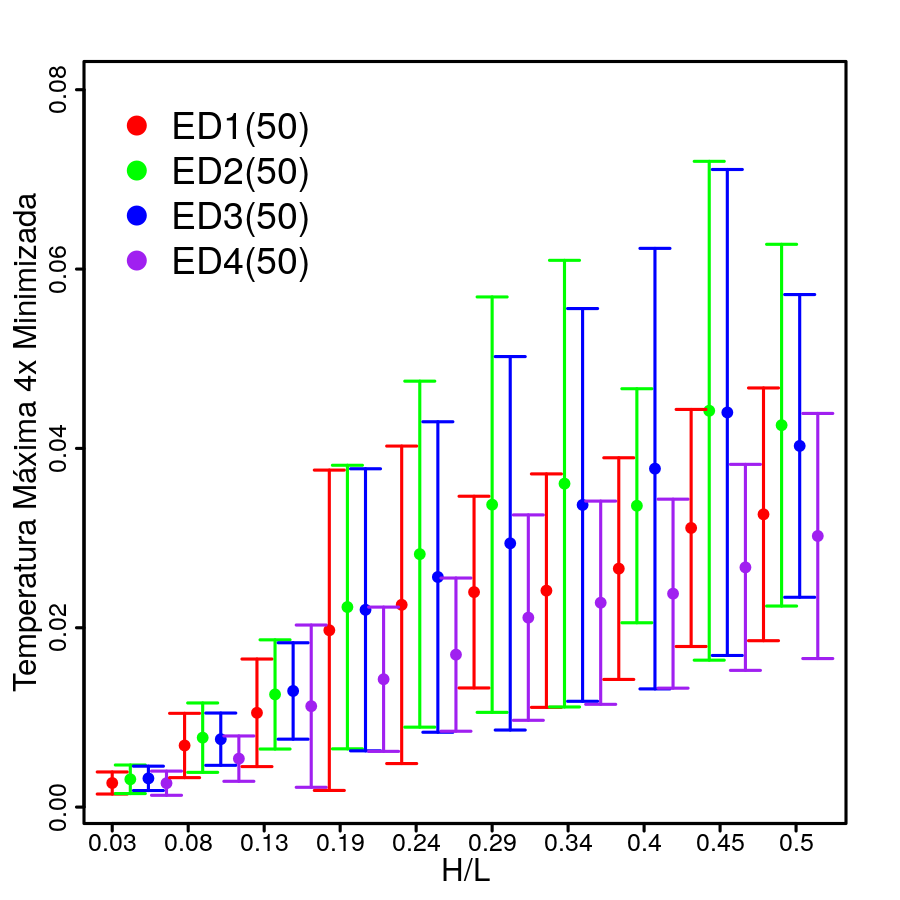
\includegraphics[scale=.98]{imgs/plot_deall50_rdata_std_003-05.png}
\quad
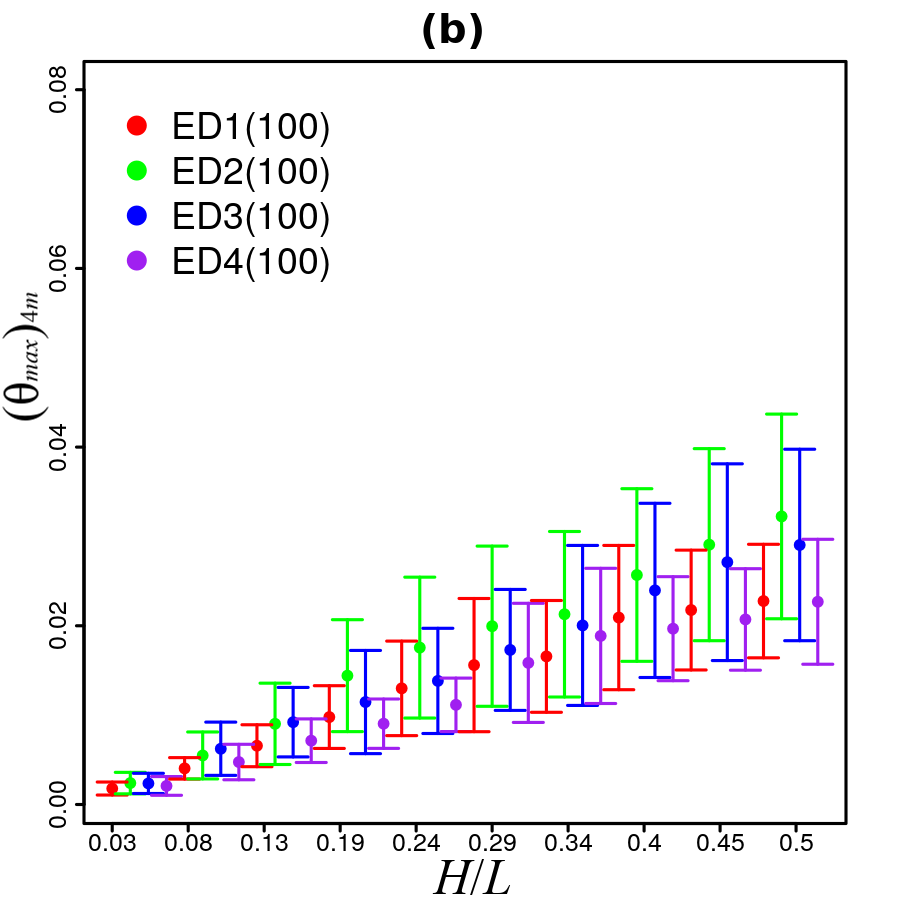
\includegraphics[scale=.98]{imgs/plot_deall100_rdata_std_003-05.png}
\quad
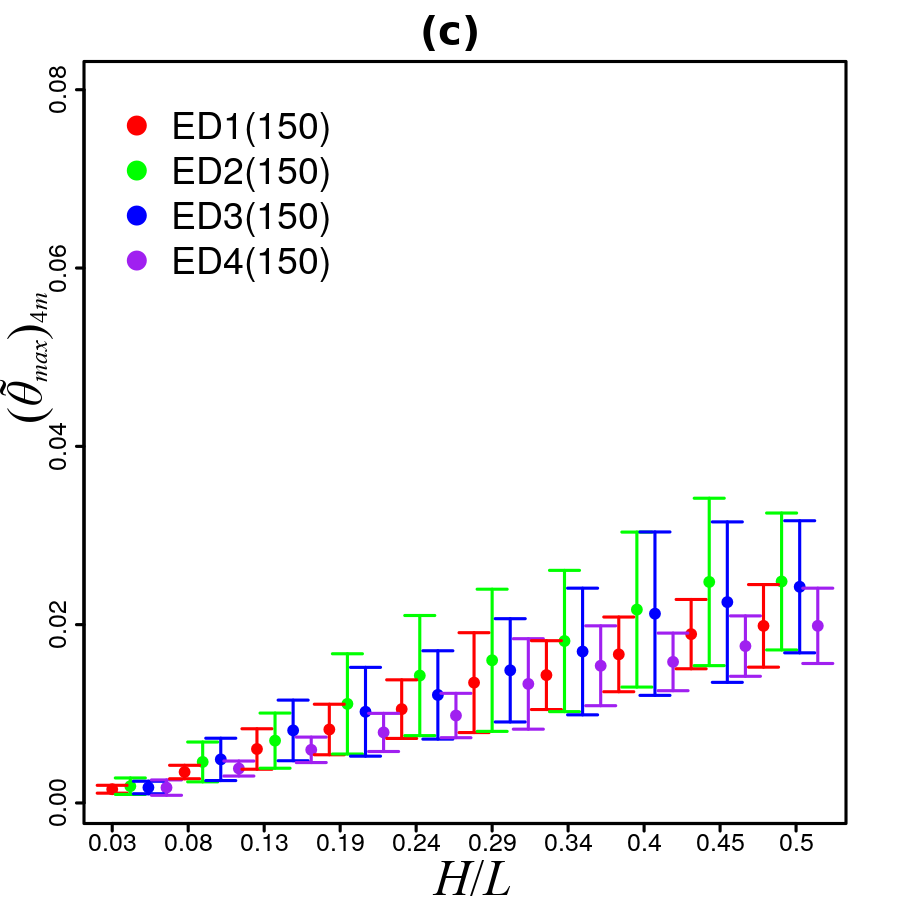
\includegraphics[scale=.98]{imgs/plot_deall150_rdata_std_003-05.png}
\quad
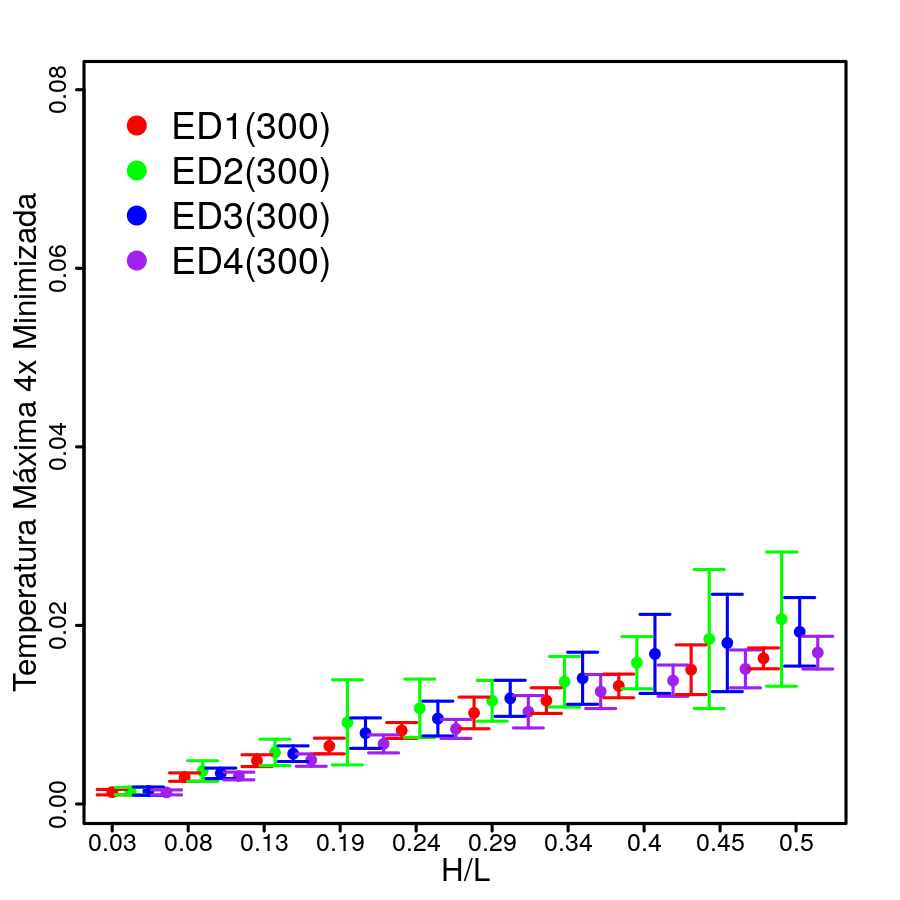
\includegraphics[scale=.98]{imgs/plot_deall300_rdata_std_003-05.png}

\caption{\fontsize{10pt}{\baselineskip}\selectfont Média e Desvio Padrão do Efeito de $H/L$ sobre $({\tilde{\theta}}_{max})_{4m}$ para $H/L\leqslant0.5$, registrados por diferentes versões do algoritmo ED com diferentes combinações de população e gerações: a)$NP=5$, $G=10$ b)$NP=10$, $G=10$ c) $NP=10$, $G=15$ d) $NP=15$, $G=20$.}
\label{stddeall}
\end{figure}

A Figura \ref{stddeall} apresenta a comparação entre as diferentes versões do algortmo ED para cada combinação dos parâmetros de  ($NP \times G$). Os resultados de diferentes algoritmos com os limites de iterações (50, 100, 150 e 300) são representados pelas figuras Fig.\ref{stddeall} (a) a Fig.\ref{stddeall} (d), respectivamente. Na Fig. \ref{stddeall} é possível observar que os algoritmos ED2 e ED3 possuem os maiores valores de desvio padrão para $({\tilde{\theta}}_{max})_{4m}$, sendo que os resultados destes algoritmos para 100 iterações são próximos aos valores de desvio padrão dos algoritmos de ED1 e ED4 com 50 iterações. O mesmo caso pode ser observado comparando os resultados apresentados na Fig. \ref{stddeall} (c) em relação a Fig. \ref{stddeall} (b), assim como, entre as Fig. \ref{stddeall} (d) e Fig. \ref{stddeall} (c), ou seja, os algoritmos ED1 e ED4 possuem maior eficiência que os algoritmos ED2 e ED3, pois apresentam o mesmo desvio padrão para um número menor de iterações. Em alguns casos, os resultados do desvio padrão de $({\tilde{\theta}}_{max})_{4m}$ do algoritmo ED2, mesmo com 300 iterações ($H/L=0.5$), o grau de dispersão é maior do que os resultados dos algoritmos ED1 e ED4, limitados as 150 iterações ($NP=10$ e $G=15$). O incremento no número de iterações dos aloritmos através das configurações dos parâmetros de população ($NP$) e gerações ($G$) contribui significativamente para a diminuição da dispersão dos resultados, principalmente entre 50 a 150 iterações. A diferença do desvio padrão entre 150 e 300 iterações diminui, principalmente para os algoritmos ED1 e ED4. A partir de 300 iterações o custo computacional não é justificável e não apresentaria um impacto relevante na dispersão dos resultados para as versões ED1 e ED4. É importante destacar que a variação no tempo de processamento entre as diferentes iterações investigadas é linear, ou seja, 300 iterações custam aproximadamente o dobro de tempo de processamento do que 150 iterações.


\hspace{0.5cm} A Figura \ref{stddegls} apresenta o resultado do efeito de $H/L$ sobre as configurações geométricas ótimas da cavidade em Duplo-T, i.e., ( ${(H_{0}/L_{0})_{4o}}$,  ${(H_{2}/L_{2})_{3o}}$, ${(H_{1}/L_{1})_{2o}}$ e ${(S_{1}/H_{0})_{o}}$). Na Fig \ref{stddegls}(a), é possível observar a dispersão e a média do efeito de  $H/L$ sobre o ${(H_{0}/L_{0})_{4o}}$. A partir desses resultados, não é possível afirmar com certeza qual o melhor algoritmo, visto que a dispersão é muito semelhante e aumenta de acordo com o aumento de $H/L$ e a magnitude de ${(H_{0}/L_{0})_{4o}}$.

\begin{figure}[htbp]
\centering
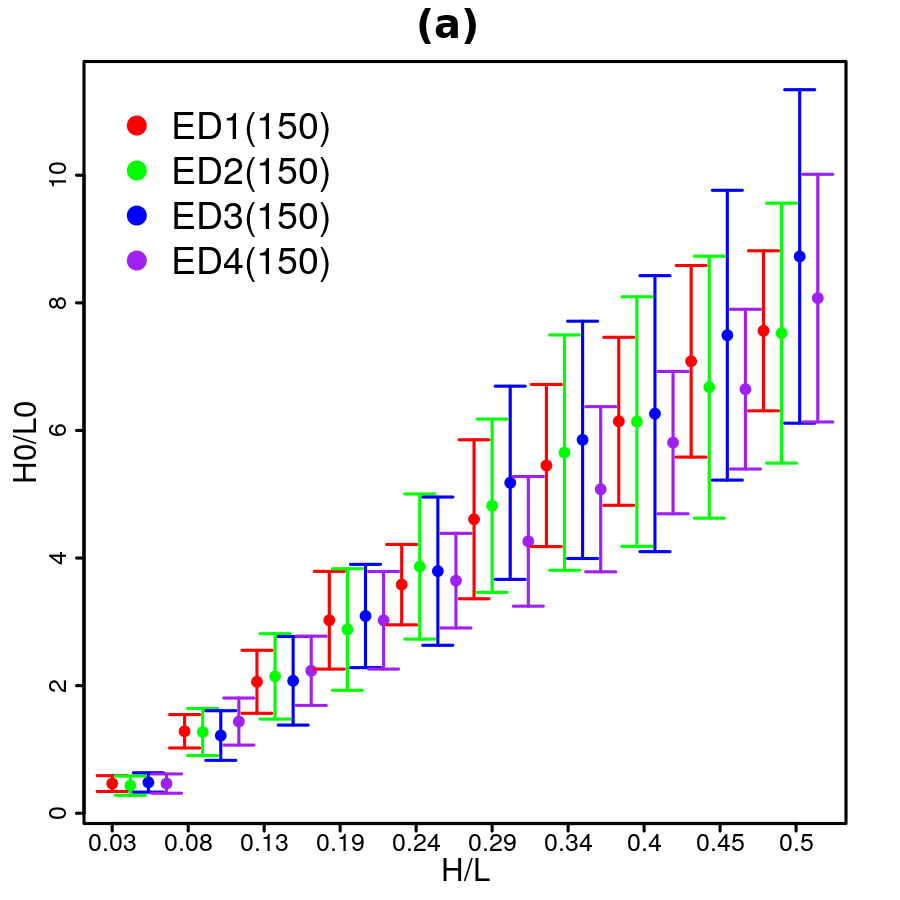
\includegraphics[scale=.98]{imgs/plot_deall150_rdata_std_h0l0.png}
\quad
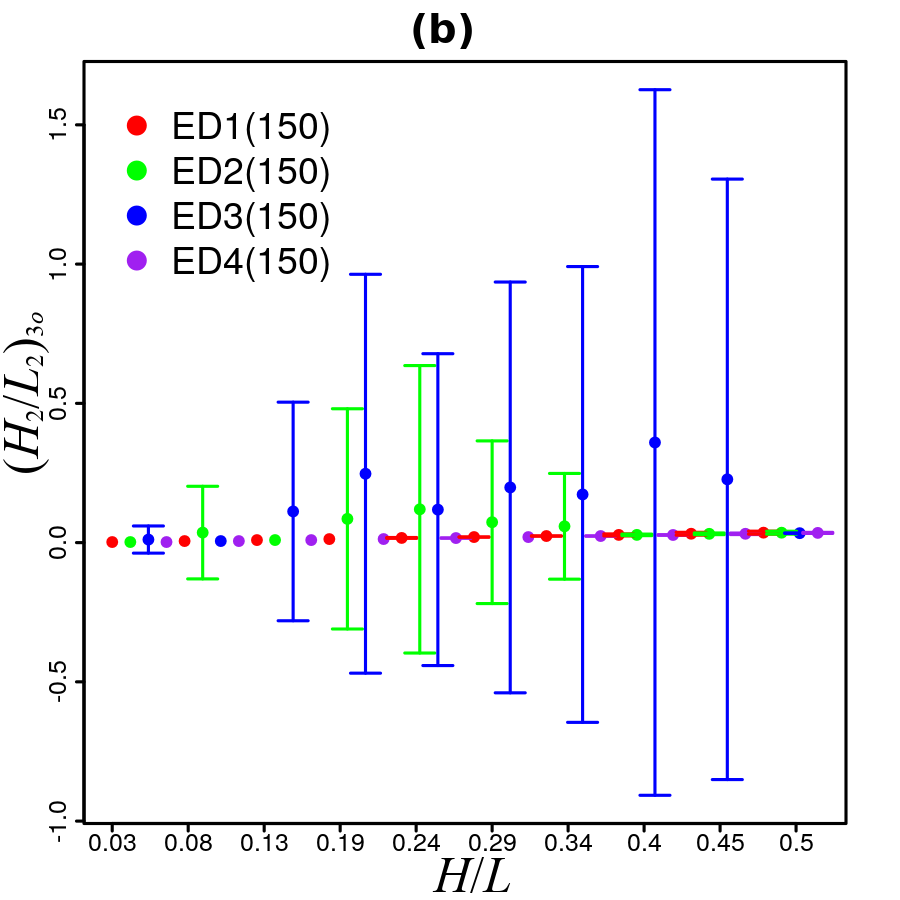
\includegraphics[scale=.98]{imgs/plot_deall150_rdata_std_h2l2.png}
\quad
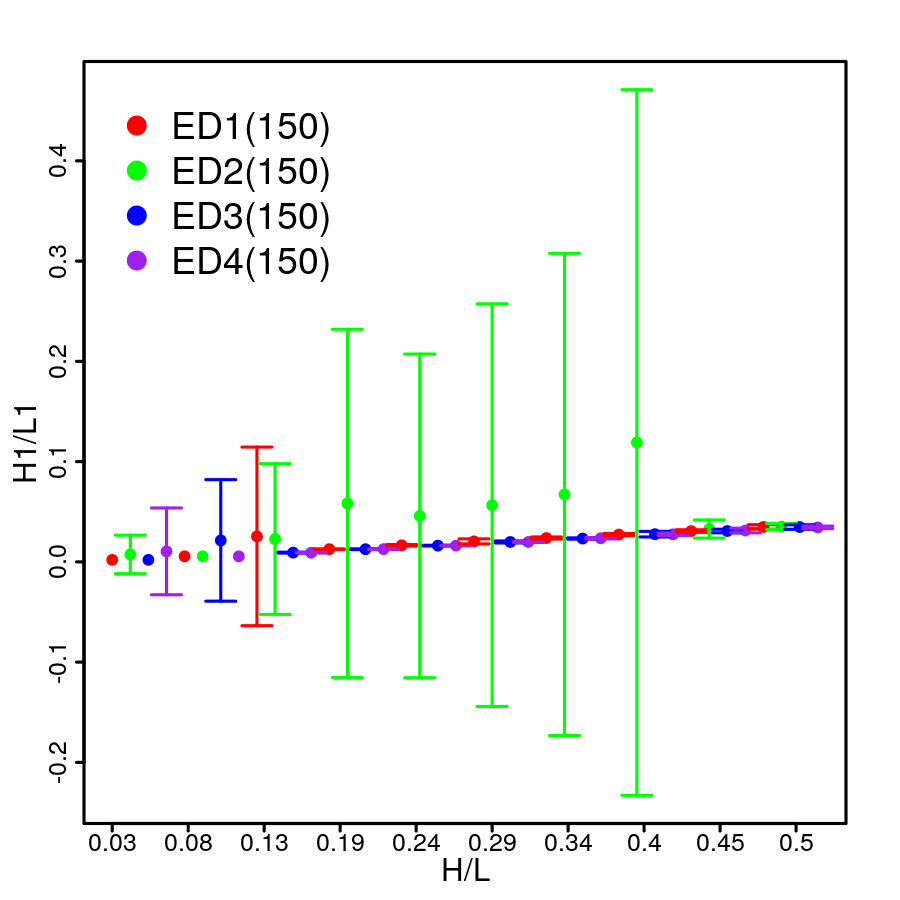
\includegraphics[scale=.98]{imgs/plot_deall150_rdata_std_h1l1.png}
\quad
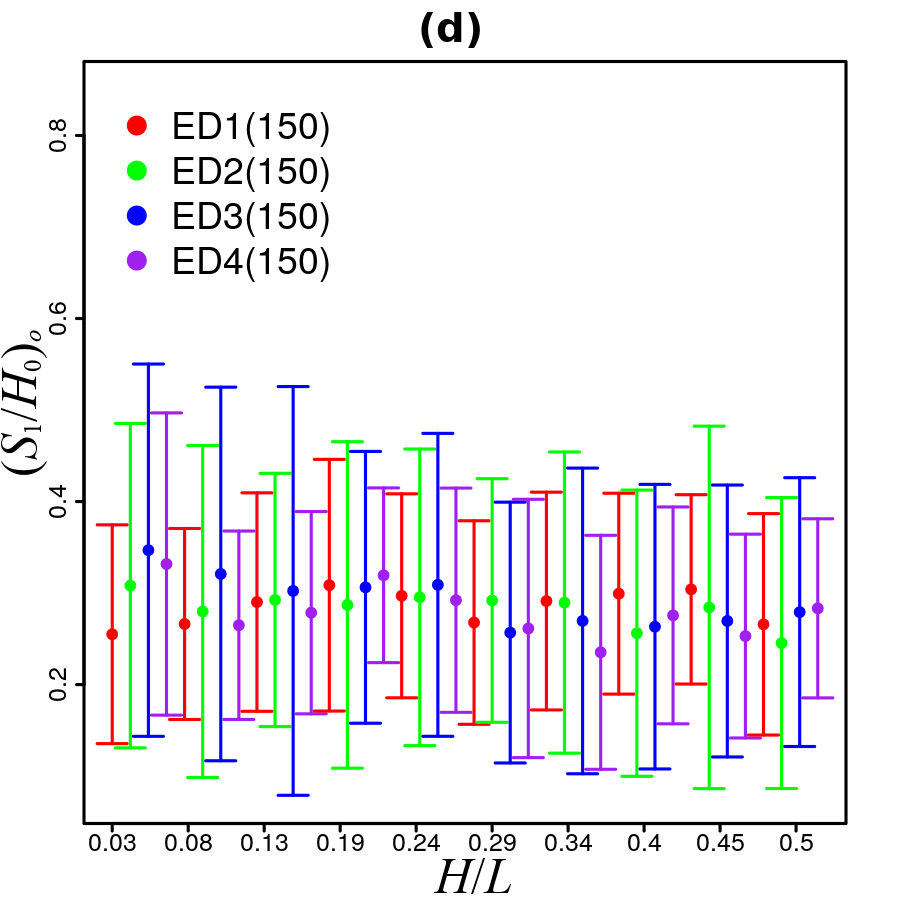
\includegraphics[scale=.98]{imgs/plot_deall150_rdata_std_s1h0.png}

\caption{\fontsize{10pt}{\baselineskip}\selectfont Média e Desvio Padrão do Efeito de $H/L$ sobre a geometria ótima, registrados por diferentes versões do algoritmo ED com limite de 150 iterações: a) Efeito de $H/L$ sobre ${(H_{0}/L_{0})_{4o}}$, b) Efeito de $H/L$ sobre ${(H_{2}/L_{2})_{3o}}$, c) Efeito de $H/L$ sobre ${(H_{1}/L_{1})_{2o}}$, d) Efeito de $H/L$ sobre ${(S_{1}/H_{0})_{o}}$.}
\label{stddegls}
\end{figure}


 De acordo com as Figuras \ref{stddegls}(a) e \ref{stddegls}(d), o desvio padrão é levemente menor para os algoritmos ED1 e ED4, mas não representa uma diferença significativa que possa alterar a interpretação dos resultados e da avaliação da geometria ótima. Entretanto, para o efeito de $H/L$ sobre ${(H_{2}/L_{2})_{3o}}$	, os algoritmos ED2 e ED3 apresentaram uma grande dispersão nos resultados, como pode ser observado na Fig. \ref{stddegls}(b). Esta situação apresenta a incapacidade dessas versões do algoritmo ED em escapar de mínimos locais.  A Fig. \ref{stddegls}(c) também apresenta uma maior dispersão dos resutlados do algoritmo ED2 para a reprodução do efeito de $H/L$ sobre ${(H_{1}/L_{1})_{2o}}$. Analisando os resultados para  ${(H_{1}/L_{1})_{2o}}$ e ${(H_{2}/L_{2})_{3o}}$, os algoritmos ED1 e ED4 novamente aparecem com o melhor desempenho, ou seja, sem dispersão nos resultados. O algorimo ED3 também apresenta um bom resultado para a otimização de ${(H_{1}/L_{1})_{2o}}$, como mostra a Fig.\ref{stddegls}(c). O efeito de $H/L$ sobre ${(S_{1}/H_{0})_{o}}$ é apresentado na Fig.\ref{stddegls}(d), através dos resultados apresentados pelas diferentes versões do algoritmo ED, não é possível determinar qual foi o mais robusto. Todas as versões apresentam uma dispersão semelhante nos resultados para este grau de liberdade, com uma pequena redução do desvio padrão nos resultados dos algoritmos ED1 e ED4, para alguns valores de $H/L$.


\section{Conclusão}
\label{opt}
\hspace{0.5cm} O presente trabalho analisou a aplicação do algoritmo de Evolução Diferencial (ED), combinado ao método de Design Construtal, para a otimização geométrica da cavidade em forma de Duplo-T. O problema possui cinco Graus de Liberdade (GL), sendo otimizados apenas quatro neste estudo ($H_{0}/L_{0}$,  $H_{2}/L_{2}$, $H_{1}/L_{1}$ e $S_{1}/H_{0}$) para diferentes valores da razão $H/L$. Este estudo avaliou o desempenho de diferentes configurações do algoritmo de ED para a determinação do efeito de $H/L$ sobre a geometria ótima e a temperatura máxima em excesso adimensional quatro vezes minimizada  $({\tilde{\theta}}_{max})_{4m}$.

A avaliação do algoritmo de ED foi concentrada nos parâmetros que configuram o comportamento do método. Portanto, foram empregadas diferentes versões do algoritmo com variações nos parâmetros de Mutação, Cruzamento ($CR$), Fator de Amplificação Diferencial ($F$), Tamanho da População ($NP$) e Número de Gerações ($G$). Quatro diferentes versões do algortimo ED foram avaliadas (ED1, ED2, ED3 e ED4), representadas na Tab. \ref{tab:algos}. Também foi analisado o número de iterações do algoritmo, representado pelos parâmetros $NP$ e $G$, de acordo com a Tab. \ref{tab:popgeracao}. Foram executadas trinta rodadas de cada versão do algoritmo ED para os diferentes limites de iterações. Os resultados da otimização foram registrados e utilizados para a análise através da média e desvio padrão dos valores da geometria ótima e da temperatura máxima em excesso adimensional quatro vezes minimizada em função da razão $H/L$.

Ao final deste estudo, e de acordo com os resultados obtidos, é possível observar a influência que os parâmetros do algoritmo de otimização podem ter sobre a avaliação geométrica. Sendo necessário, portanto, a especialização destes parâmetros ao problema de interesse. Para o problema de otimização da cavidade em forma de Duplo-T, os resultados indicam que as verões ED1 e ED4 possuem o melhor desempenho. Estas versões apresentaram, na grande maioria dos casos investigados, a menor dispersão e portanto a reprodução mais adequada do efeito de $H/L$ sobre o desempenho térmico da cavidade. As configurações de parâmetros em comum entre estas duas versões do ED ($CR=0.7$, $F=1.5$), sugerem que estes são os parâmetros mais apropriados ao problema de interesse.

%**********************************************************************************
\section*{Agradecimentos}
\hspace{0.5cm}G. V. Gonzales agradece o IF-SUL e o  PPGMC-FURG pelo apoio. E. D. dos Santos agradece o suporte financeiro do CNPq. Antônio J. Silva Neto agradece o suporte financeiro da FAPERJ, CNPq e CAPES.
%**********************************************************************************

%\bibliographystyle{apacite}
\bibliographystyle{mcsul}
\bibliography{referencial}
\end{document}